\documentclass[12pt, a4paper]{article}

\setlength{\oddsidemargin}{0.5cm}
\setlength{\evensidemargin}{0.5cm}
\setlength{\topmargin}{-1.6cm}
\setlength{\leftmargin}{0.5cm}
\setlength{\rightmargin}{0.5cm}
\setlength{\textheight}{24.00cm} 
\setlength{\textwidth}{15.00cm}
\setcounter{tocdepth}{4}
\setcounter{secnumdepth}{4}
\parindent 0pt
\parskip 5pt
\pagestyle{plain}

\usepackage{multirow}
\usepackage[bottom]{footmisc}
\usepackage{listings}
\usepackage{graphicx}
\graphicspath{{./images/}}

\title{Predicting Mental Imagery Concreteness}
\author{Mark Angelo Gabriel\\[0.5cm]{\small Advisors: Dr. Julie Ji, Dr. Wei Liu, Dr Francisco De Toni}}
\date{}

\newcommand{\namelistlabel}[1]{\mbox{#1}\hfil}
\newenvironment{namelist}[1]{%1
\begin{list}{}
    {
        \let\makelabel\namelistlabel
        \settowidth{\labelwidth}{#1}
        \setlength{\leftmargin}{1.1\labelwidth}
    }
  }{%1
\end{list}}

\begin{document}
\maketitle

\tableofcontents
\listoffigures
\listoftables


\section{Abstract} The COVID-19 pandemic has forced a sudden change in society that we weren't fully prepared for.  Self-isolation and physical distancing has been imposed on everyone in varying degrees and the effect of it on people's mental wellbeing is an area of interest, especially if a second or third wave of the pandemic will require people to undergo isolation again. Certain members of the community are going to be affected more than others from this rapid disruption of the day-to-day because they are not getting the usual levels of social interaction they need or are used to to maintain a healthy mental wellbeing. It is in our interest to find which members of our community are at most risk with a method that is highly accessible given the physical restrictions that such a societal condition imposes. 

Mental imagery, the simulation of perceptual experience across sensory modalities, has been strongly linked to depression. It is one avenue that we may attempt to examine a person on to see if they are at risk of suffering from loneliness. Inference and prediction of a person's quality of mental imagery, particularly concreteness, is the focus of this research. Classical techniques and natural language processing techniques have been employed to generate a series of models to understand mental imagery concreteness. 

\section{Review of Literature}

\subsection{Mental Imagery}
Mental imagery is the simulation of perceptual experience \cite{Kosslyn2001} across sensory modalities. It has been strongly linked to depression \cite{Patel2005} which is our main area of interest. As detailed in Kosslyn et al's 2001 paper, the current techniques for measurements of a person's mental imagery involve visual tests, classification tasks, comparison tasks, questionnaires and interviews. 

The usage of machine learning and natural language processing has not yet been deeply explored in extracting mental imagery parameters, though theoretically, it would be most similar to the existing method of using interviews and analyzing a person's speech and selection of words to derive the wanted parameters, except with machine learning, the assessment would be automated rather than needing a trained professional to go through each case individually, which would be an expensive process that won't be easily scalable in an isolation scenario where potentially a huge percentage of people are affected.

Dr. Julie Ji's research on mental imagery, the experience of perception in the absence of external sensory input, shows that the person's quality of mental imagery-based simulations has a significant link to maintaining and amplifying emotional states \cite{conceptualandclinical}. In one study on mental imagery as a motivational amplifier to promote activities as a key treatment in depression \cite{motivationalamplifier}, the Motivational Imagery group reported higher levels of motivation, anticipated pleasure, and anticipated reward for the planned activities compared to the Activity Reminder control group and the No-Reminder control group.

\subsection{Named Entity Recognition}
We aim to be able to utilise the free-text responses of the survey to create a model that performs better than a regression model from the human-graded mental imagery parameters that predicts a person's risk of loneliness. To achieve this, the collected free-text responses have to be annotated with respect to the domain of interest. In our particular research area, it will be important to tag self actions (meditate, jog, sleep in, watch TV, etc) and interpersonal actions (call friend, video call with parents, have dinner at restaurant with partner) separately, which most pre-trained models aren't trained to do. Due to this, and also because we have a relatively small sample size, we have the luxury of using manual annotation to improve our data's richness and context.

In the paper Multilingual Twitter Sentiment Classification: The Role of Human Annotators by Mozetic et al, \cite{Mozeti__2016}, they find that the quality of classification models depends much more on the quality and size of training data than on the type of model trained. Human annotators can help us maximise our model's performance by ensuring good annotation quality, which can be done by setting an overlap value (the number of times a single corpus is annotated) of at least 2.


\begin{figure}
	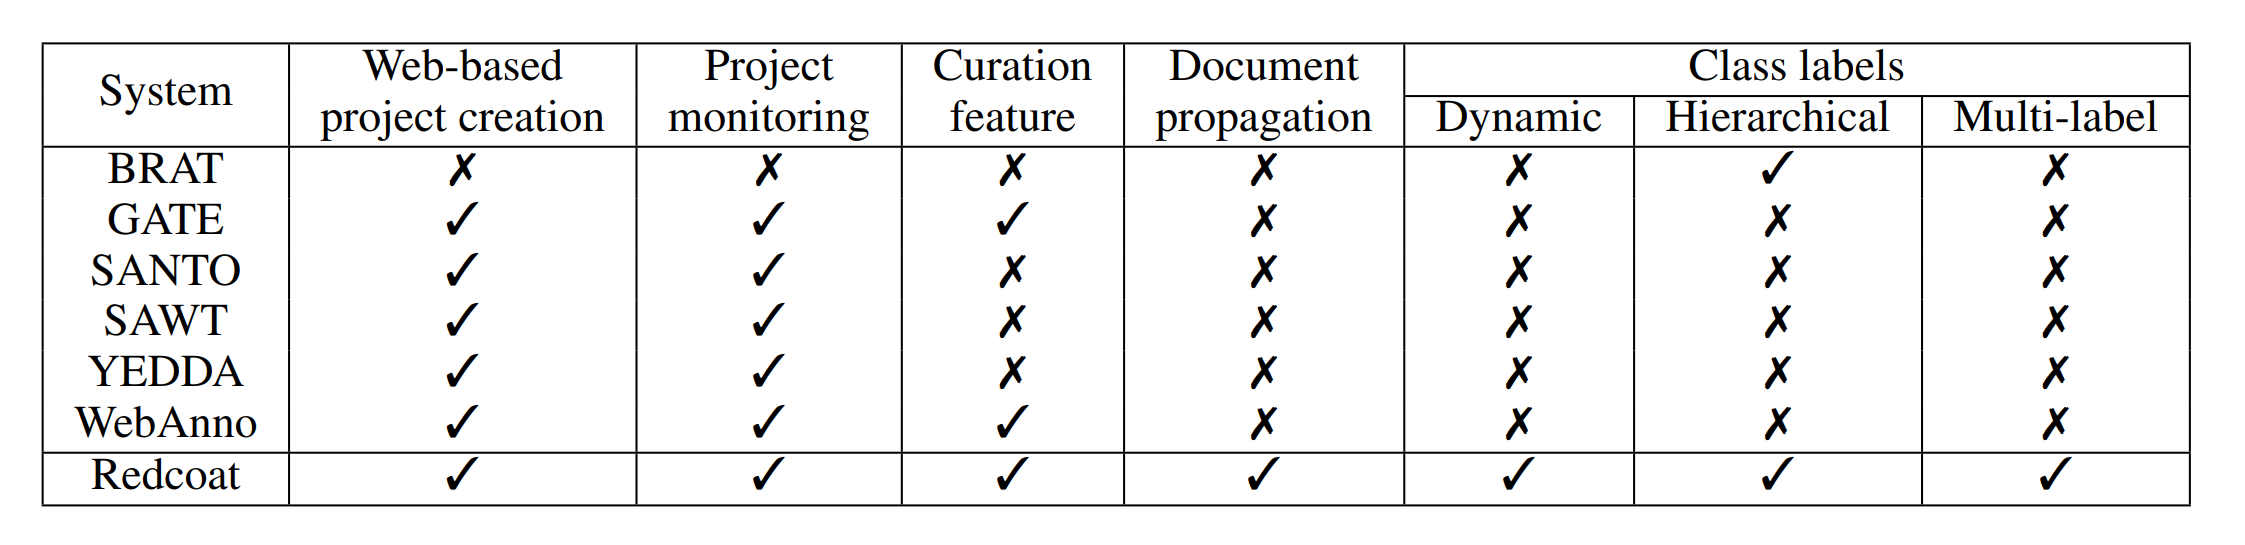
\includegraphics[scale=0.25]{annotating_tools}
	\caption{Annotation tools comparison}
	\label{annot_table}
\end{figure}

There are a lot of tools for data annotation available. Among these options are BRAT, GATE Teamware, WebAnno, SAWT, Yedda, SANTO and UWA's Redcoat. We can see a comparison of their features in Figure \ref{annot_table}. With research assistants to help out with our data as annotators, an important feature we are looking for in an annotating tool is the ability to propagate documents easily and for the tool to scale the workload automatically based on the number of annotators.  Redcoat \cite{stewart-etal-2019-redcoat} has been selected as the annotating tool for that reason, alongside being web-based and easy to set up and distribute. 

\subsection{Sentiment Analysis}
One of the mental imagery parameters we're concerned with is a person's emotional tone when they're describing what they think or see when they're given a scenario and a goal of starting lonely in an isolated setting and ending in a brighter, happier mental state. A person's emotional tone can be approximated with sentiment analysis techniques. XLNet has been used to identify optimism and pessimism in twitter messages by Alshahrani et al \cite{alshahrani2019xlnet}, which is similar to what we're trying to achieve. XLNet models are able to model negations and other semantic relationships by paying attention to key words, leading to a model accuracy of 0.9645. 

A point of discussion would be if our research problem would work better with basic sentiment analysis or aspect-based sentiment analysis. Normal sentiment analysis grades the emotional tone of the overall text, while aspect-based sentiment analysis goes through the text to identify various aspects and determines the corresponding emotional tone for each one. There isn't much available literature on when each of the techniques are relevant or when each of them should be used over the other, but the spirit of parsimony would lead us to towards using aspect-based sentiment analysis only if there are particular aspects in our research domain that we want to track individually. 

For the lack of literature on comparison between the two techniques on different domains, there is merit in trying both individually, or creating a model that uses both techniques in tandem and empirically comparing which technique works best for our research problem.

\subsection{Transfer Learning}
Language is complex. In order to get reasonably performing models from scratch, one would need an extremely large dataset in addition to the computing power needed to process it. This is often impossible for many researchers, and a solution to this problem is transfer learning. Transfer learning is a machine learning technique where a model is trained on a particular problem, then reused in a similar domain to carry over the knowledge of the neural network. Depending on how different the pre-trained model is to your problem, Additional training needs to be done to finetune the model to your specific domain. \cite{ruder2019transfer}

Popular pre-trained NLP models include Google's BERT, Google and Carnegie Mellon University's XLNet, and Facebook's RoBERTa. All of these models are transformers which are deep learning models designed to handle sequential data using the concept of attention mechanisms. Attention mechanisms allow the model to access and use any previous states and utilises them based on relevance to the current node. \cite{vaswani2017attention} 

In particular, we want a pretrained model that is strong in sentiment analysis. Looking at Figure \ref{benchmarks} in the SST-2 column which stands for the Stanford Sentiment Treebank v2, we can see that XLNet \cite{yang2020xlnet} outperforms both BERT and RoBERTa in sentiment analysis on the SST-2 dataset.

While XLNet, BERT and RoBERTa all come from the same family of models, XLNet differs by introducing permutation language modelling, where all tokens are predicted in a random, permutated order rather than the traditional sequential order. This helps XLNet learn non-adjacent and bidirectional relationships between the words in the corpus. Secondly, XLNet uses Transformer-XLs as the base architecture which enables learning dependency beyond a fixed length without disrupting temporal coherence. \cite{dai2019transformerxl} Transformer-XLs, even without the permutation language modelling, has been shown to give performance increases in NLP tasks. 

\begin{figure}
	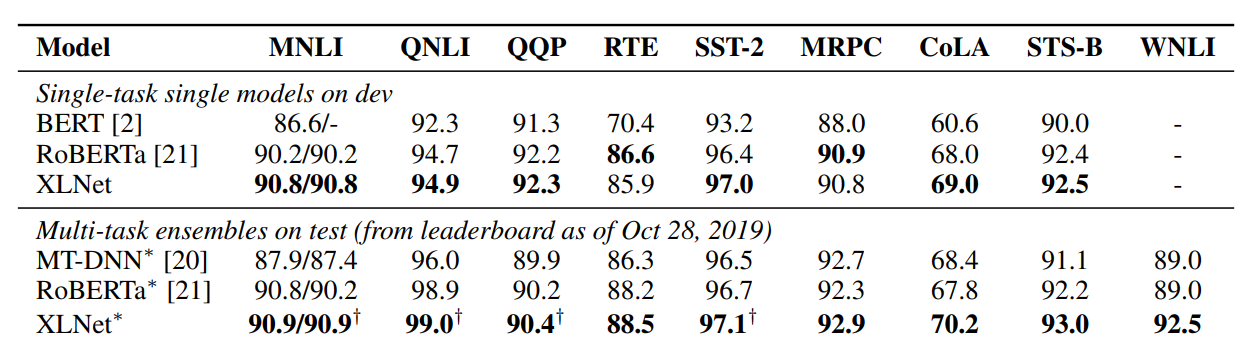
\includegraphics[scale=0.45]{benchmarks}
	\caption{Pre-trained NLP models results on GLUE}
	\label{benchmarks}
\end{figure}

For the above reasons, and for the benchmarks set out in Figure \ref{benchmarks}, XLNet will be our pretrained model of choice. In addition, HuggingFace \cite{Wolf2019HuggingFacesTS} provides a transformer library that wraps all of these transformers for use with PyTorch or TensorFlow in a neat package that allows us to utilise the base XLNet model and the large XLNet model, alongside any other pretrained transformer model if we wish to make model comparisons. 

\section{Data}

\subsection{Core dataset}
The core dataset for this study is a conglomerate of surveys from volunteers (n=1269) including a baseline day zero survey, daily surveys, and weekly checkpoints up to the fourteenth day. The baseline survey asked for the volunteers' mental health status, education, employment, age, coinhabitant count, isolation experience, the Hospital Anxiety and Depression Scale (HADS) scores, and other miscellaneous information. A loneliness score and social activity score have been assigned to each volunteer based on their answers to the relevant questions. In addition, a text response to the below instruction was requested. 

\begin{quote}
The story begins with you feeling isolated and lonely.

The story ends with you feeling connected and closer to people.

Please come up with the steps you would take to achieve the story ending, providing as much detail as you can about your thoughts, feelings, and actions related to these problem-solving steps.
\end{quote}

The responses are then manually rated by humans on four mental imagery parameters. Each response is assessed by two raters to improve reliability. The final score is calculated as the average of the two ratings. The four mental imagery parameters are as below:

\begin{itemize}
  \item Number of relevant problem-solving steps: Discrete steps that helps the person to reach the desired goal or to overcome an obstacle along the way
  \item Solution Effectiveness: How much you think the described solution would maximise positive and minimise negative consequences in the short-term and long-term, both personally and socially
  \item Solution Concreteness: The degree to which the described solution reflects concrete plans, i.e. involving specific actions, times, places, and people
  \item Emotional Tone: The degree to which the participant sounds negative (downbeat/pessimistic/unsure) or positive (upbeat/optimistic/confident)
\end{itemize}

The daily surveys track the the volunteers' depression and anxiety levels, their Warwick-Edinburgh Mental Well-being Scale (WEMWBS) scores, physical activity levels,  social activity levels, and if and how often they've been outside of their accommodation. The weekly surveys include the normal daily survey questions and adds HADS, loneliness, and optimism score assessments.

\subsection{Word concreteness dataset}
The paper \textit{Predicting Word Concreteness and Imagery} \cite{charbonnier-wartena-2019-predicting} by Charbonnier and Wartena has outputted a dictionary of words and their concreteness ratings. These scores are obtained by training a regression model using precomputed word embeddings from GoogleNews and fastText, suffixes and the word's part of speech (POS) tag as the features and manually scored concreteness values as the target. The dataset contains 39955 unique singleton and bigram words.

\subsection{Discretisation of Concreteness}
Concreteness is recorded as a numerical number between 1 and 5 with half steps and some quarter steps in between due to the averaging done on the varying ratings on some of the observations. Given our dataset is small (n=1236, 1088 if you remove invalid responses), it is of interest to further decrease the number of bins for Concreteness. It will also help with the interpretation of the model, as in practice, we will be looking for people with generally low, medium or high concreteness values, not necessarily if they have a score of 1 or 1.5. 

\begin{figure}[ht]
\centerline{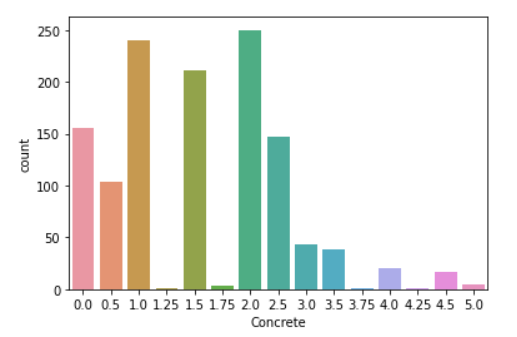
\includegraphics[scale=0.8]{concreteness_distribution.png}}
\caption{Concreteness histogram}
\label{concreteness_distribution}
\end{figure}
 
Three levels have been deemed important in the scope of this research: Low, Medium, and High. The cutoff points were chosen to minimise the relative class sizes, as if we were to trisect the number scale, we would end up with a high class imbalance particularly against High. See Figure \ref{concreteness_distribution}to see the raw concreteness distribution. Concreteness scores in the [0, 1.5) range are classed into Low, [1.5, 2.5) into Medium, and [2.5, 5] into High. While the number of observations falling under High Concreteness is still fairly lower than those in Low or Medium as can be seen in Figure \ref{concreteness_discrete_distribution}, any other cutoff combination for our dataset would make further imbalance the classes. This is just the nature of our data where concreteness scores are concentrated in the lower ranges.

Aside from the three levels, we will also explore models focusing on a boolean classification of Low Concreteness or not. 

\begin{figure}
\centerline{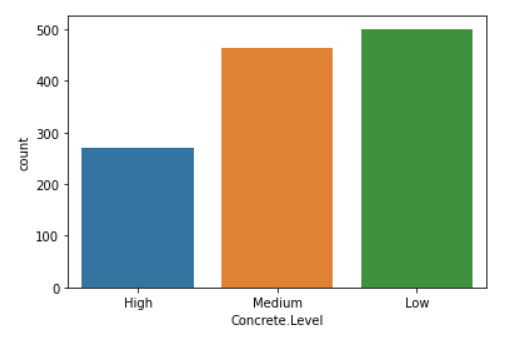
\includegraphics[scale=0.8]{concreteness_discrete_distribution.png}}
\caption{Discretised Concreteness histogram}
\label{concreteness_discrete_distribution}
\end{figure}

\section{Methodology}

\subsection{Inferential analysis}

The goal for this section is to discover key features in the data that can be easy identifiers for concreteness without resorting to unexplainable prediction models. It would be valuable to know particular features of low and high concreteness individuals as it may give us a better understanding on the subject matter.

\subsubsection{Baseline model}
The baseline model will be a predictor model for concreteness from non-textual information available from a candidate at day zero. Information such as loneliness and social activity scores available at future days will not be accessible to this model. Its purpose is to find out how accurate we can get our predictions to be of concreteness given a person's own profile, demographic, and self-assessment alone. The full list of parameters used for this baseline model is itemised below: 

\begin{itemize}
  \item Demographical information: age, gender, education, employment, and working from home status
  \item Self-rated assessments of mental imagery in terms of actions, people, emotions, and vividness
  \item Number and type of cohabitants, including pets
  \item HADS scores for depression and anxiety calculated through a series of questions
  \item Number of days practicing social distancing to date
  \item Perceived risk of loneliness, worry, stress, family conflict, inactivity and listlessness
  \item If any current or past mental health diagnoses exist

\end{itemize}

Stepwise selection will be used to narrow down the predictive parameters to only the most significant few to maximise the AIC score of the model. Multiple linear regression will be the regression technique of choice in order to better understand the effect of each significant variable on concreteness as compared to less inferential techniques such as support vector machines. 

\subsubsection{Word-level mined variables}
Word-level approaches will be applied to the response texts to gather high level information to see if non-NLP text approaches can bring an improvement in performance to our Concreteness prediction model. Primarily, the word concreteness dictionary from Charbonnier's \textit{Predicting Word Concreteness and Imagery} paper \cite{charbonnier-wartena-2019-predicting} will be utilised to gather new features from the responses in our observations. Bigrams will also be included in the data mining.

Multiple linear regression will be used similar to the baseline model, with the difference being the addition of new data on word concreteness. Stepwise selection will be used to narrow down the predictive parameters, with the new fields being added to the model afterwards if not already selected by the algorithm. 


\subsubsection{One-vs-rest Classification}
The discretisation of Concreteness will allow us to use the One-vs-rest logistic classification. Three individual models will be created for predicting if an observation is of Low, Medium, or High Concreteness. This will also make it possible to see if different factors count for different Concreteness levels which may come useful for inference of what variables to look out for for specific classes. 

Stratified sampling will be done for the train test split as it is important to make sure that each class is relatively equally represented given the slight imbalance in class sizes.

\subsubsection{Decision Tree}
Decision Trees are highly explainable classification models which could give us heuristics for classifying a person's level of Concreteness. We will be using Conditional Inference Trees \cite{ctree} using the \lstinline{ctree} command  from the \lstinline{party} package in R.

\subsection{Prediction with natural language processing techniques}

\subsubsection{BERT pretrained model}
BERT (Bidirectional Encoder Representations from Transformers) \cite{bert} is a popular application of bidirectional training of transformers to language modelling. Transfer learning has been shown to be extremely valuable especially on small datasets such as in this study, and we are interested to see what kind of performance improvements we will see with using BERT pretrained models in a feed forward neural network ending with three nodes representing the three concreteness classes with a softmax layer applied at the end for classification.

In addition, we will try to augment the model above with the high concreteness word count variable to see if it will further push the performance upwards.

\subsubsection{BiLSTM Classifier}

\subsubsection{Transformer model with XLNet}

\subsection{Prediction with classical techniques}

\subsubsection{SVM Classifier}

\subsubsection{Random Forest Classifier}

\subsubsection{XGBoost Classifier}
\subsection{Summary}

\section{Results and Discussion}

\subsection{Inferential analysis}

\subsubsection{Baseline model}
Using the stepwise algorithm for model selection on linear regression has yielded the following model:

\begin{table}[ht]
\centering
\begin{tabular}{||c c c c||} 
 \hline
 Coefficient & Estimate & Standard Error & p-value \\ [0.5ex] 
 \hline\hline
 Intercept & 0.7309 & 0.4178 & 0.0806 \\ 
 Perceived Risk (Listlessness) & -0.1065 & 0.0298 & 0.0004 \\
 Self-rated Mental Imagery Score (Action)  & 0.0798 & 0.0289 & 0.0058 \\
 Coinhabitants (Adult, Other)\footnotemark & -0.1901 & 0.0798 & 0.0175 \\
 Mental Health Diagnosis (none) & 0.8957 & 0.4099 & 0.0291 \\ 
Mental Health Diagnosis (unsure) & 1.2529 & 0.4995 & 0.0123 \\
Mental Health Diagnosis (yes - current) & 0.9820 & 0.4133 & 0.0177 \\
Mental Health Diagnosis (yes - past) & 0.0485 & 0.0314 & 0.1226\\
 Self-rated Mental Imagery Score (Vividness)  & 0.0485 & 0.0314 & 0.1226 \\ [1ex] 
 \hline
\end{tabular}
\caption{Baseline Model}
\label{table:1}
\end{table}
\footnotetext{Number of adult coinhabitants that aren't your family, partner, or friend.}

This baseline model has an adjusted $R^2$ score of $0.0400$ which means that the variables selected account only for approximately 4\% of the variance of Concreteness, which is abysmally low and unusable for prediction purposes. This low score can  mean two possible things. First is that the relationship between the predictors and the target variable may not be linear in nature. Second is that the baseline variables may simply not be strongly related to a person's concreteness of mental imagery that is estimated by humans by assessing the response text.  

\subsubsection{Word-level mined variables}
A series of new fields have been generated using the word concreteness dictionary from Charbonnier's \textit{Predicting Word Concreteness and Imagery} paper \cite{charbonnier-wartena-2019-predicting}. Concreteness information from both individual words and bigrams have been mined. Raw counts and densities (raw count over total word count) were obtained for both high concreteness (defined by having a score of greater than three in an approximate five point scale) and extreme concreteness (defined by having a score of greater than four in an approximate five point scale) for individual words. Raw counts for high concreteness is the only metric obtained for bigrams as there are generally fewer tagged bigrams to score in the corpus. Raw word count has also been added.

Using the stepwise algorithm for model selection on linear regression has yielded the following model:

\begin{table}[ht]
\centering
\begin{tabular}{||c c c c||} 
 \hline
 Coefficient & Estimate & Standard Error & p-value \\ [0.5ex] 
 \hline\hline
 Intercept & 1.5834 & 0.1033 & $<$ 2e-16 \\ 
 High Concreteness Word Count\footnotemark & 0.0191 & 0.0050 & 0.0001 \\
 Perceived Risk (Listlessness) & -0.0865 & 0.0268 & 0.0013 \\
 Self-rated Mental Imagery Score (Vivid)  & 0.0552 & 0.0273 & 0.0435 \\
 Outside Activity Score & -0.0550 & 0.0330 & 0.0961 \\ 
 Word Count  & -0.0016 & 0.0011 & 0.1534 \\ [1ex] 
 \hline
\end{tabular}
\caption{Word-level model}
\label{table:2}
\end{table}
\footnotetext{Number of words that have concreteness values of three or above in an approximate five point scale.}

This word-level model has an adjusted $R^2$ score of $0.0774$ which means that the variables selected account only for approximately 7.74\% of the variance of Concreteness. This is considerably higher than the baseline model's adjusted $R^2$ score of $0.0400$, but it is still inadequate for practical applications. It is valuable, however, to note that the contribution of word-level mined variables into the model nearly equals the effect of everything else in the model, which gives us further evidence to explore the text response of the observations using NLP techniques.
 
\subsubsection{One-vs-rest Classification}

A one-vs-rest classification approach has been applied to the data. This will also be useful to see if people with low levels of concreteness can be identified by different predictors to people with high levels of concreteness. A higher score in the individual models means that it is more likely that an observation belongs to the model's designated class.

\paragraph{Low Concreteness model}

\begin{table}[ht]
\centering
\begin{tabular}{||c c c c||} 
 \hline
 Coefficient & Estimate & Standard Error & p-value \\ [0.5ex] 
 \hline\hline
 Intercept & -0.0874 & 0.2159 & 0.6856 \\ 
 High Concreteness Word Count & -0.0469 & 0.0078 & 1.77e-09 \\
 Perceived Risk (Listlessness)  & 0.1847 & 0.0739 & 0.0125 \\ [1ex] 
 \hline
\end{tabular}
\caption{Low Concreteness Model}
\label{table:low}
\end{table}

The model parameters can be found in Table \ref{table:low}. The low concreteness model has yielded a training accuracy of 0.6758 and a test accuracy of 0.72. This model is the simplest one we've encountered which is quite insightful. Both high concreteness word count and perceived risk of listlessness are consistently significant predictors for many of our models here, and the patterns are the same. More occurences of high concreteness words generally lead to high concreteness scores (hence the negative relationship between high concreteness word counts and the probability of being a low concreteness observation) and a higher perceived risk of listlessness generally leads to low concreteness scores.

\paragraph{Medium Concreteness model}

\begin{table}[ht]
\centering
\begin{tabular}{||c c c c||} 
 \hline
 Coefficient & Estimate & Standard Error & p-value \\ [0.5ex] 
 \hline\hline
 Intercept & -1.0859 & 0.3971 & 0.0063 \\ 
 High Concreteness Bigram Count & -0.2209 & 0.1079 & 0.0407 \\
 Distancing Impact  & 0.0854 & 0.0512 & 0.0950 \\ 
 Isolation Days & -0.0145 & 0.0093 & 0.1216 \\ 
 Age Group (25-44)  & 0.5346 & 0.3739 & 0.1527 \\ 
 Age Group (45-64)  & 0.4569 & 0.3580 & 0.2019 \\
 Age Group (65-79)  & 0.9387 & 0.3858 & 0.0150 \\
 Age Group (80+)  & 1.3443 & 0.9836 & 0.1717 \\
 Physical Activity Score  & 0.0144 & 0.0094 & 0.1245 \\ [1ex] 
 \hline
\end{tabular}
\caption{Medium Concreteness Model}
\label{table:medium}
\end{table}

The model parameters can be found in Table \ref{table:medium}. The medium concreteness model has yielded a training accuracy of 0.5710 and a test accuracy of 0.5086. This model is the worst performer of the one-vs-rest models, sitting just a small bit better than guessing if an observation counts as a medium concreteness observation or not. Luckily, predicting low and high concreteness observations are more important in practical applications. 

\paragraph{High Concreteness model}

\begin{table}[ht]
\centering
\begin{tabular}{||c c c c||} 
 \hline
 Coefficient & Estimate & Standard Error & p-value \\ [0.5ex] 
 \hline\hline
 Intercept & -1.6622 & 0.3240 & 2.88e-07 \\ 
 High Concreteness Word Count & 0.0601 & 0.0157 & 0.0001 \\
 Word Count & -0.0067 & 0.0034 & 0.0513 \\
 High Concreteness Bigram Count & 0.2446 & 0.1242 & 0.0488 \\
 Perceived Risk (Listlessness)  & -0.2000 & 0.0875 & 0.0223 \\ 
 Self-rated Mental Imagery Score (Scenes)  & 0.1394 & 0.0776 & 0.0723 \\ 
 Working From Home (No)  & -0.6766 & 0.2724 & 0.0130 \\ 
 Working From Home (Yes, some work days)  & -0.1932 & 0.3338 & 0.5626 \\ 
 Working From Home (Yes, all work days)  & 0.1008 & 0.2330 & 0.6652 \\ 
 Coinhabitants (Children)  & 0.1707 & 0.1019 & 0.0939 \\ 
 Distancing Impact  & -0.1031 & 0.0659 & 0.1176 \\ [1ex] 
 \hline
\end{tabular}
\caption{High Concreteness Model}
\label{table:high}
\end{table}

The model parameters can be found in Table \ref{table:high}. The high concreteness model has yielded a training accuracy of 0.7762 and a test accuracy of 0.7771. From the relatively high accuracy scores, it seems like high concreteness observations are more easily predictable with our given variables. High concreteness word and bigram count appear as significant variables, with the negative estimate on word count working as a balancer to divide responses rich in high concreteness words as compared to responses that are just long. Perceived risk of listlessness is also present, staying consistent in its negative relationship to concreteness.

\paragraph{Concreteness Classifier}

A concreteness classifier that uses the outputs of the three individual models and selects the max has been created. A confusion matrix on the model's predictions on the test dataset can be found on Table \ref{table:onevall}. Its overall accuracy is 0.4571 which still is low for practical usage. The statistics by class can be found in Table \ref{table:onevallstats}.

\begin{table}[ht]
\centering
\begin{tabular}{l|l|c|c|c|c}
\multicolumn{2}{c}{}&\multicolumn{3}{c}{True level}&\\
\cline{3-5}
\multicolumn{2}{c|}{}&Low&Medium&High&\multicolumn{1}{c}{Total}\\
\cline{2-5}
\multirow{3}{*}{Predicted level}& Low & 18 & 15 & 3 & 36\\
\cline{2-5}
& Medium & 34 & 52 & 29 & 115\\
\cline{2-5}
& High & 5 & 9 & 10 & 24\\
\cline{2-5}
\multicolumn{1}{c}{} & \multicolumn{1}{c}{Total} & \multicolumn{1}{c}{57} & \multicolumn{    1}{c}{76} & \multicolumn{    1}{c}{42} & \multicolumn{1}{c}{175}\\
\end{tabular}
\caption{One-vs-rest Classifier}
\label{table:onevall}
\end{table}

\begin{table}[ht]
\centering
\begin{tabular}{||c c c c||} 
 \hline
 Statistic & Low & Medium & High \\ [0.5ex] 
 \hline\hline
 Sensitivity & 0.3158 & 0.6842 & 0.2381 \\ 
 Specificity & 0.8475 & 0.3636 & 0.8947 \\
 Prevalence & 0.3257 & 0.4343 & 0.2400 \\
 Detection Rate & 0.1029 & 0.2971 & 0.0571 \\
 Detection Prevalence  & 0.2057 & 0.6571 & 0.1371 \\ 
 Balanced Accuracy  & 0.5816 & 0.5239 & 0.5664 \\ [1ex] 
 \hline
\end{tabular}
\caption{One-vs-rest Statistics by Class}
\label{table:onevallstats}
\end{table}

\subsubsection{Decision Tree}

A conditional inference tree as specified in Hothorn, Hornik, and Zeileis's paper \cite{ctree} has yielded the decision tree in Figure \ref{decision_tree}. A confusion matrix on the model's predictions on the test dataset can be found on Table \ref{table:decision_tree}. Its overall accuracy is 0.4663 which still is low for practical usage, but slightly better than the one-vs-rest classifier which is impressive considering the tree is minimalistic in its choice of nodes. The statistics by class can be found in Table \ref{table:decisiontreestats}. 

\begin{figure}[ht]
\centerline{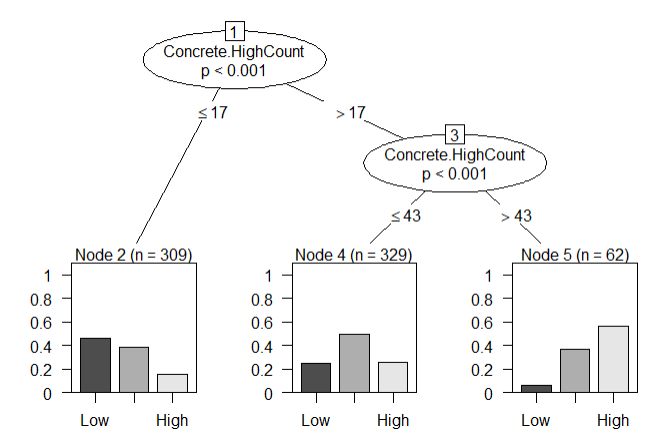
\includegraphics[scale=0.8]{decision_tree.png}}
\caption{Concreteness Decision Tree}
\label{decision_tree}
\end{figure}

\begin{table}[ht]
\centering
\begin{tabular}{l|l|c|c|c|c}
\multicolumn{2}{c}{}&\multicolumn{3}{c}{True level}&\\
\cline{3-5}
\multicolumn{2}{c|}{}&Low&Medium&High&\multicolumn{1}{c}{Total}\\
\cline{2-5}
\multirow{3}{*}{Predicted level}& Low & 28 & 30 & 9 & 67\\
\cline{2-5}
& Medium & 28 & 46 & 25 & 99\\
\cline{2-5}
& High & 2 & 1 & 9 & 12\\
\cline{2-5}
\multicolumn{1}{c}{} & \multicolumn{1}{c}{Total} & \multicolumn{1}{c}{58} & \multicolumn{    1}{c}{77} & \multicolumn{    1}{c}{43} & \multicolumn{1}{c}{178}\\
\end{tabular}
\caption{Decision Tree}
\label{table:decision_tree}
\end{table}

\begin{table}[ht]
\centering
\begin{tabular}{||c c c c||} 
 \hline
 Statistic & Low & Medium & High \\ [0.5ex] 
 \hline\hline
 Sensitivity & 0.4828 & 0.5974 & 0.2093 \\ 
 Specificity & 0.6750 & 0.4752 & 0.9778 \\
 Prevalence & 0.3258 & 0.4326 & 0.2416 \\
 Detection Rate & 0.1573 & 0.2584 & 0.0506 \\
 Detection Prevalence  & 0.3764 & 0.5562 & 0.0674 \\ 
 Balanced Accuracy  & 0.5789 & 0.5363 & 0.5935 \\ [1ex] 
 \hline

\end{tabular}
\caption{Decision Tree Statistics by Class}
\label{table:decisiontreestats}
\end{table}

The importance of the count of high concreteness words have repeatedly shown up in many of our tested models which gives a strong indication that using NLP techniques on our response might yield rich information not usually attainable with other methods.

\subsection{Prediction with natural language processing techniques}

\subsubsection{BERT Pretrained models}
The bert-base-cased pretrained model has been selected for this study. The training time has been set to 15 epochs. The first feed forward neural network created has the following layers: 

\begin{enumerate}
  \item Input layer as tokenised document using the BertTokenizer ran through the BERT pretrained model
  \item A dropout layer with probability 0.3
  \item A linear layer diluting the 768 features of the BERT layer into 3 nodes
\end{enumerate}

The second feed forward neural network is similar but adds a step in between that appends the high concreteness word count as an extra feature. An argument can be made for removing the dropout layer given that we have a small dataset and not making use of as much learning as we could from it would not be ideal, however, removing the dropout layer has shown decreased performance.. 

The first network has achieved a test accuracy of 0.4404, while the second network with the added high concreteness word count variables has achieved a test accuracy of 0.4679.

\begin{table}[ht]
\centering
\begin{tabular}{l|l|c|c|c|c}
\multicolumn{2}{c}{}&\multicolumn{3}{c}{True level}&\\
\cline{3-5}
\multicolumn{2}{c|}{}&Low&Medium&High&\multicolumn{1}{c}{Total}\\
\cline{2-5}
\multirow{3}{*}{Predicted level}& Low & 15 & 12 & 4 & 31\\
\cline{2-5}
& Medium & 17 & 30 & 20 & 67\\
\cline{2-5}
& High & 4 & 4 & 3 & 11\\
\cline{2-5}
\multicolumn{1}{c}{} & \multicolumn{1}{c}{Total} & \multicolumn{1}{c}{36} & \multicolumn{    1}{c}{46} & \multicolumn{    1}{c}{27} & \multicolumn{1}{c}{109}\\
\end{tabular}
\caption{BERT Pretrained Model}
\label{table:pretrained}
\end{table}

\begin{table}[ht]
\centering
\begin{tabular}{l|l|c|c|c|c}
\multicolumn{2}{c}{}&\multicolumn{3}{c}{True level}&\\
\cline{3-5}
\multicolumn{2}{c|}{}&Low&Medium&High&\multicolumn{1}{c}{Total}\\
\cline{2-5}
\multirow{3}{*}{Predicted level}& Low & 11 & 7 & 1 & 19\\
\cline{2-5}
& Medium & 24 & 32 & 18 & 74\\
\cline{2-5}
& High & 1 & 7 & 8 & 16\\
\cline{2-5}
\multicolumn{1}{c}{} & \multicolumn{1}{c}{Total} & \multicolumn{1}{c}{36} & \multicolumn{    1}{c}{46} & \multicolumn{    1}{c}{27} & \multicolumn{1}{c}{109}\\
\end{tabular}
\caption{BERT Pretrained Model with High Concreteness Word Count}
\label{table:pretrained2}
\end{table}

\subsubsection{BiLSTM Classifier}

\subsubsection{Transformer model with XLNet}

\subsection{Prediction with classical techniques}

\subsubsection{SVM Classifier}

\subsubsection{Random Forest Classifier}

\subsubsection{XGBoost Classifier}

\subsection{Summary}

\bibliographystyle{plain}
\bibliography{dissertation}

\end{document}

